%!TEX root = ../main.tex
\section{Results}
\subsection{Rolling correlations}
\begin{figure}[H]
  \caption{Rolling correlations on weekly data - Value factors vs. all factors}
  \label{diag:rolling45}
  % \toprule
  \centering
  \begin{minipage}{\textwidth}
  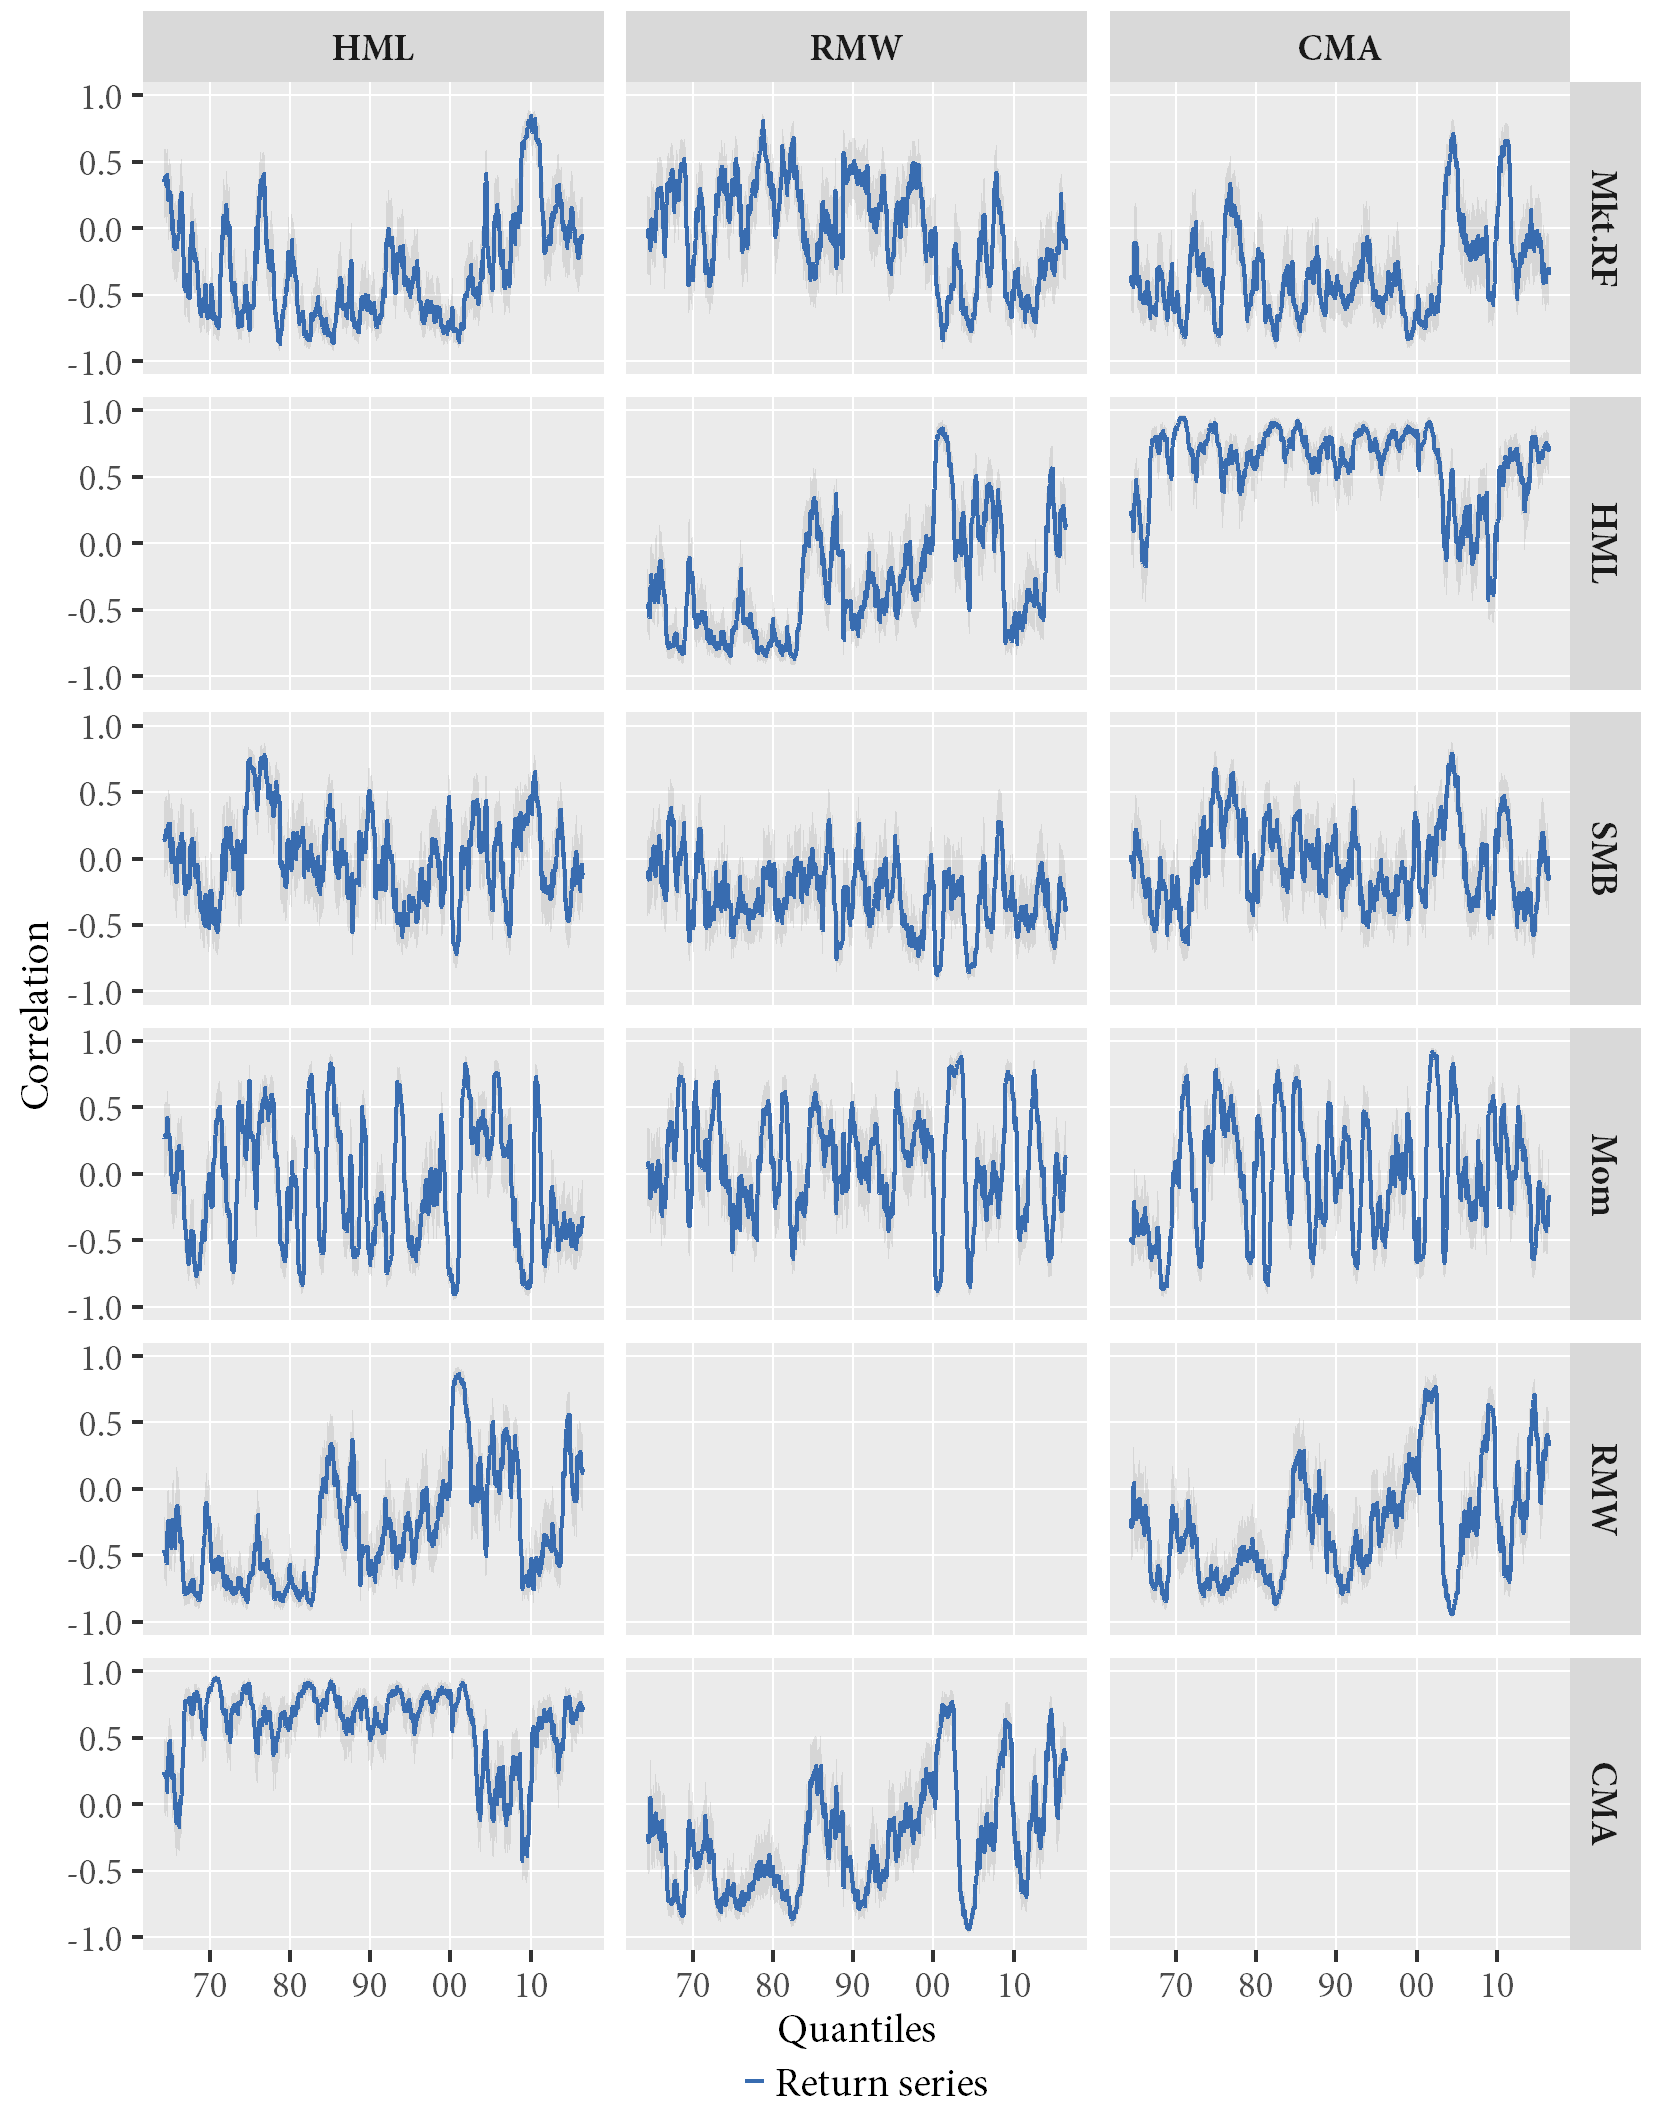
\includegraphics[scale=1]{graphics/rolling45.png}  
  % \bottomrule
  \vspace{3mm}
  \footnotesize
  We report rolling 45-week correlations of factor strategy pairs. Return series are weekly log returns. Value factors in columns and all factors in rows. Standard correlation coefficient annoted $r$ in graphs. All data 1963-07-05 - 2016-07-01.
  \end{minipage}
\end{figure}
\begin{itemize}
  \item We note that correlations are highly time-varying. Results unchanged if using residuals. Calls for a copula model that can incorporate time variation
\end{itemize}
\subsection{Threshold correlations}
\begin{figure}[H]
  \caption{Threshold correlations on weekly data - Value factors vs. non-value factors}
  \label{diag:thresholdnonvalue}
  % \toprule
  \centering
  \begin{minipage}{\textwidth}
  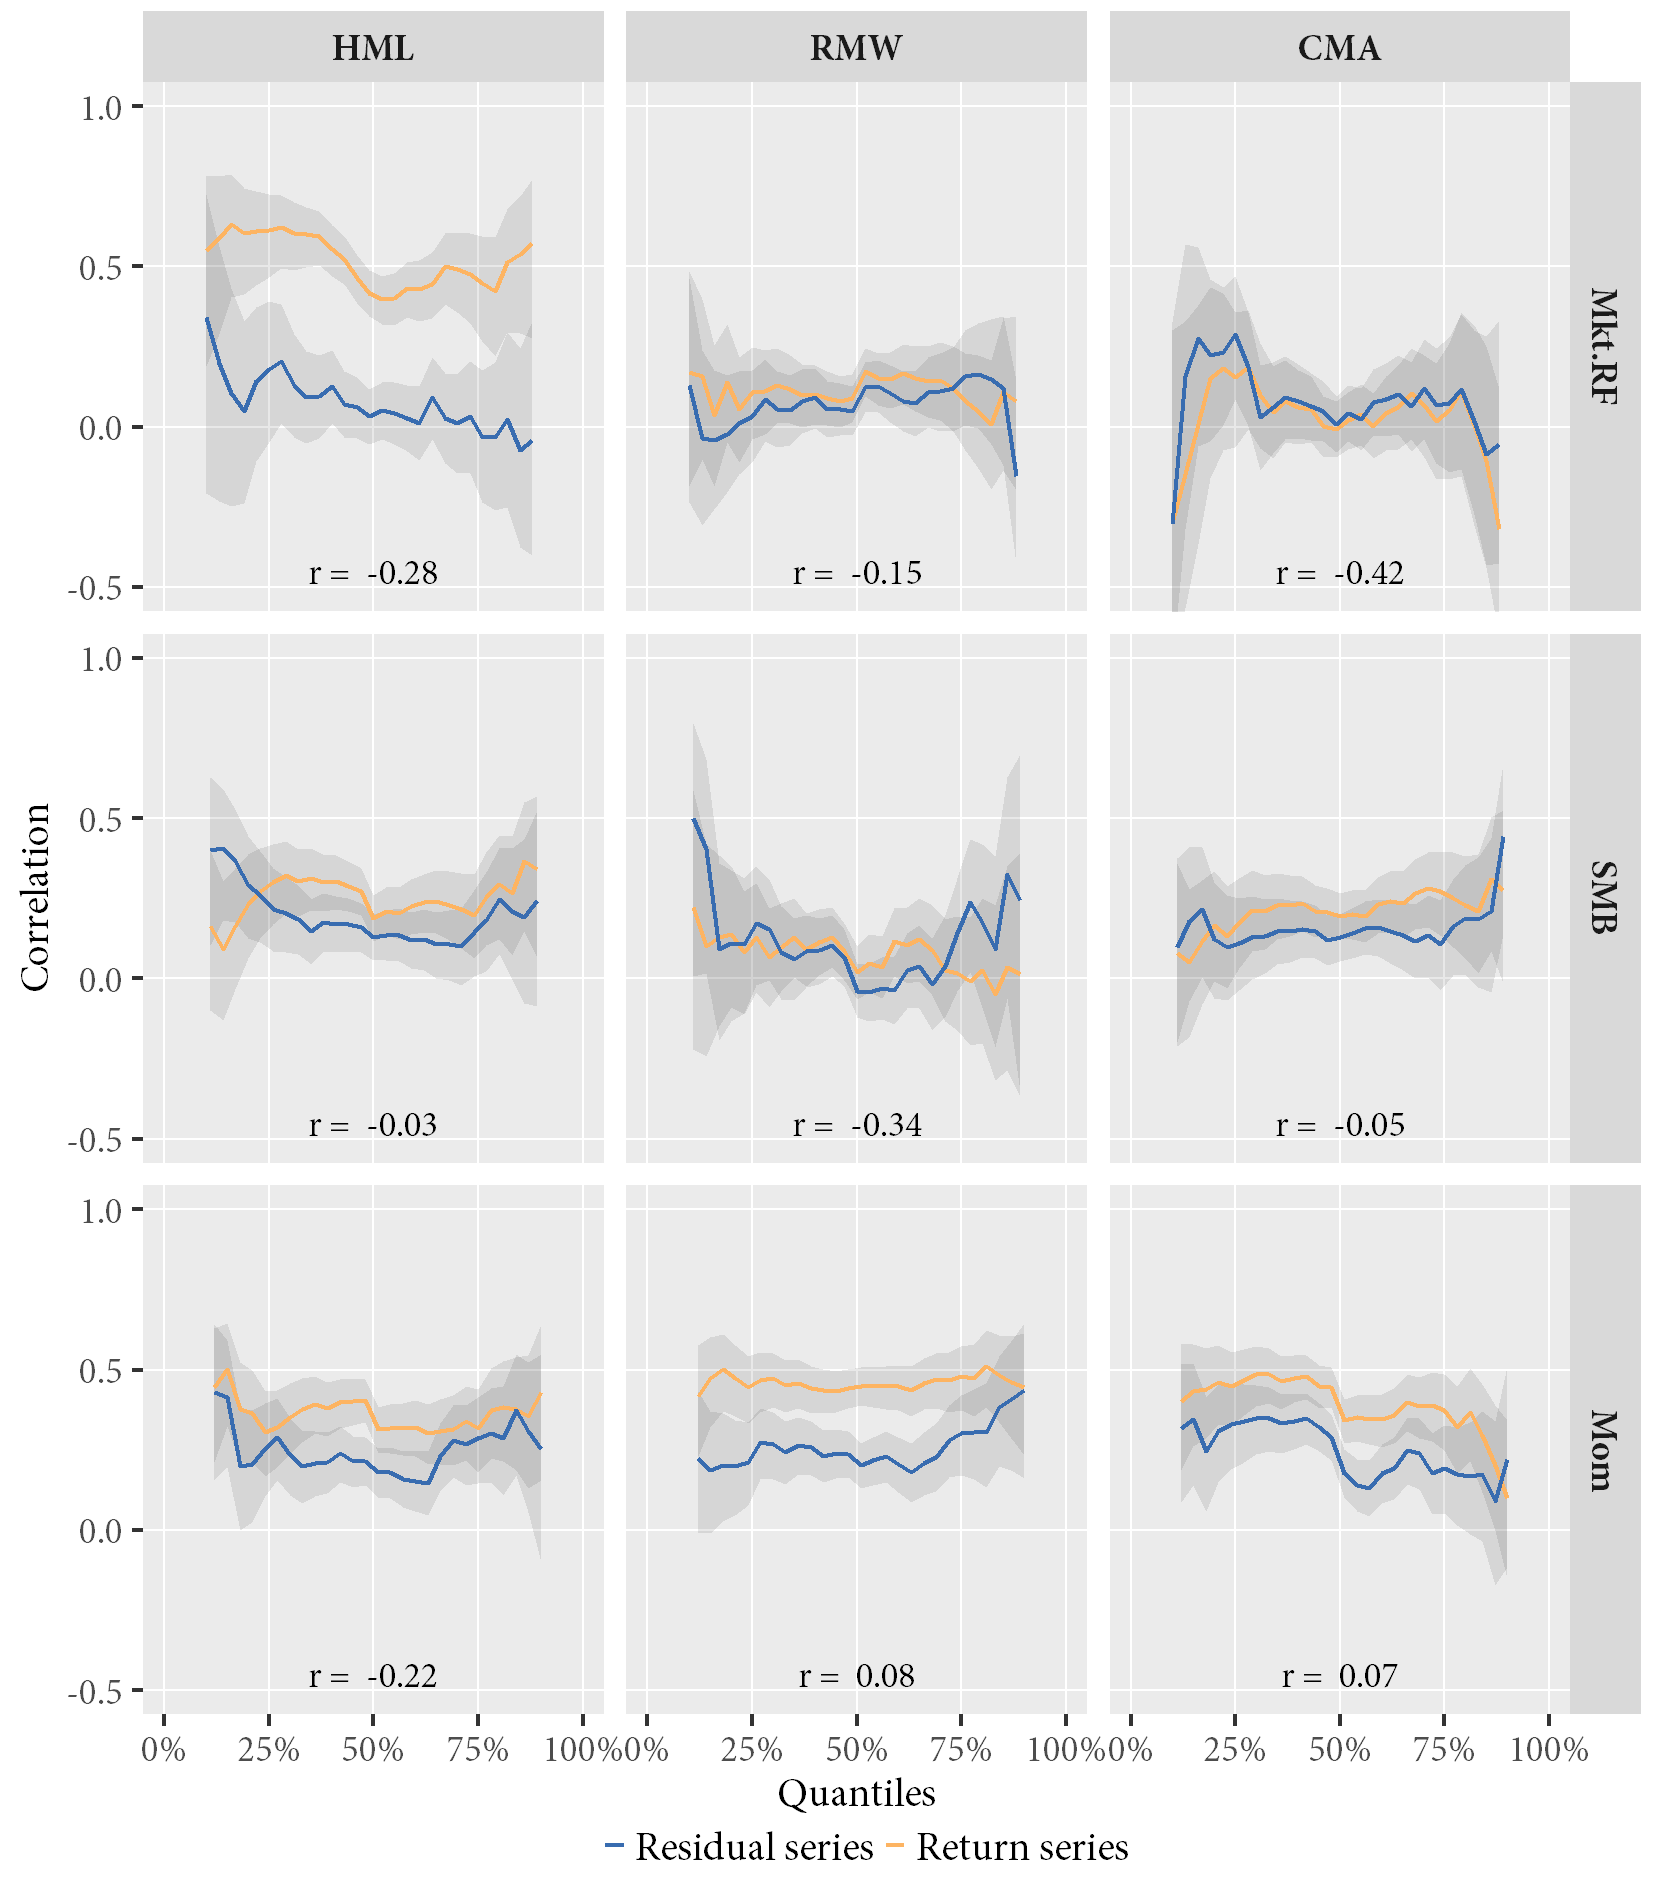
\includegraphics[scale=1]{graphics/threshold_Nonvalue.png}  
  % \bottomrule
  \vspace{3mm}
  \footnotesize
  We report threshold correlations of factor strategy pairs. Return series are weekly log returns and residual series are weekly standardized residuals from an ARMA-GJR-GARCH process. Value factors in columns and non-value factors in rows. Standard correlation coefficient annoted $r$ in graphs. All data 1963-07-05 - 2016-07-01. Correlations from 10-90\% reported, due to limited data availablility in the tails. Threshold correlations are calculated as: $Corr(r_i, r_j \,|\, r_i < F_i^{-1}(p), r_j < F_j^{-1}(p)) \text{ for } p < 0.5$ and $Corr(r_i, r_j \,|\, r_i \geq F_i^{-1}(p), r_j \geq F_j^{-1}(p)) \text{ for } p \geq 0.5$ 
  \end{minipage}
\end{figure}
\begin{figure}[H]
  \caption{Threshold correlations on weekly data - Value factors vs. themselves}
  \label{diag:thresholdvalue}
  % \toprule
  \centering
  \begin{minipage}{\textwidth}
  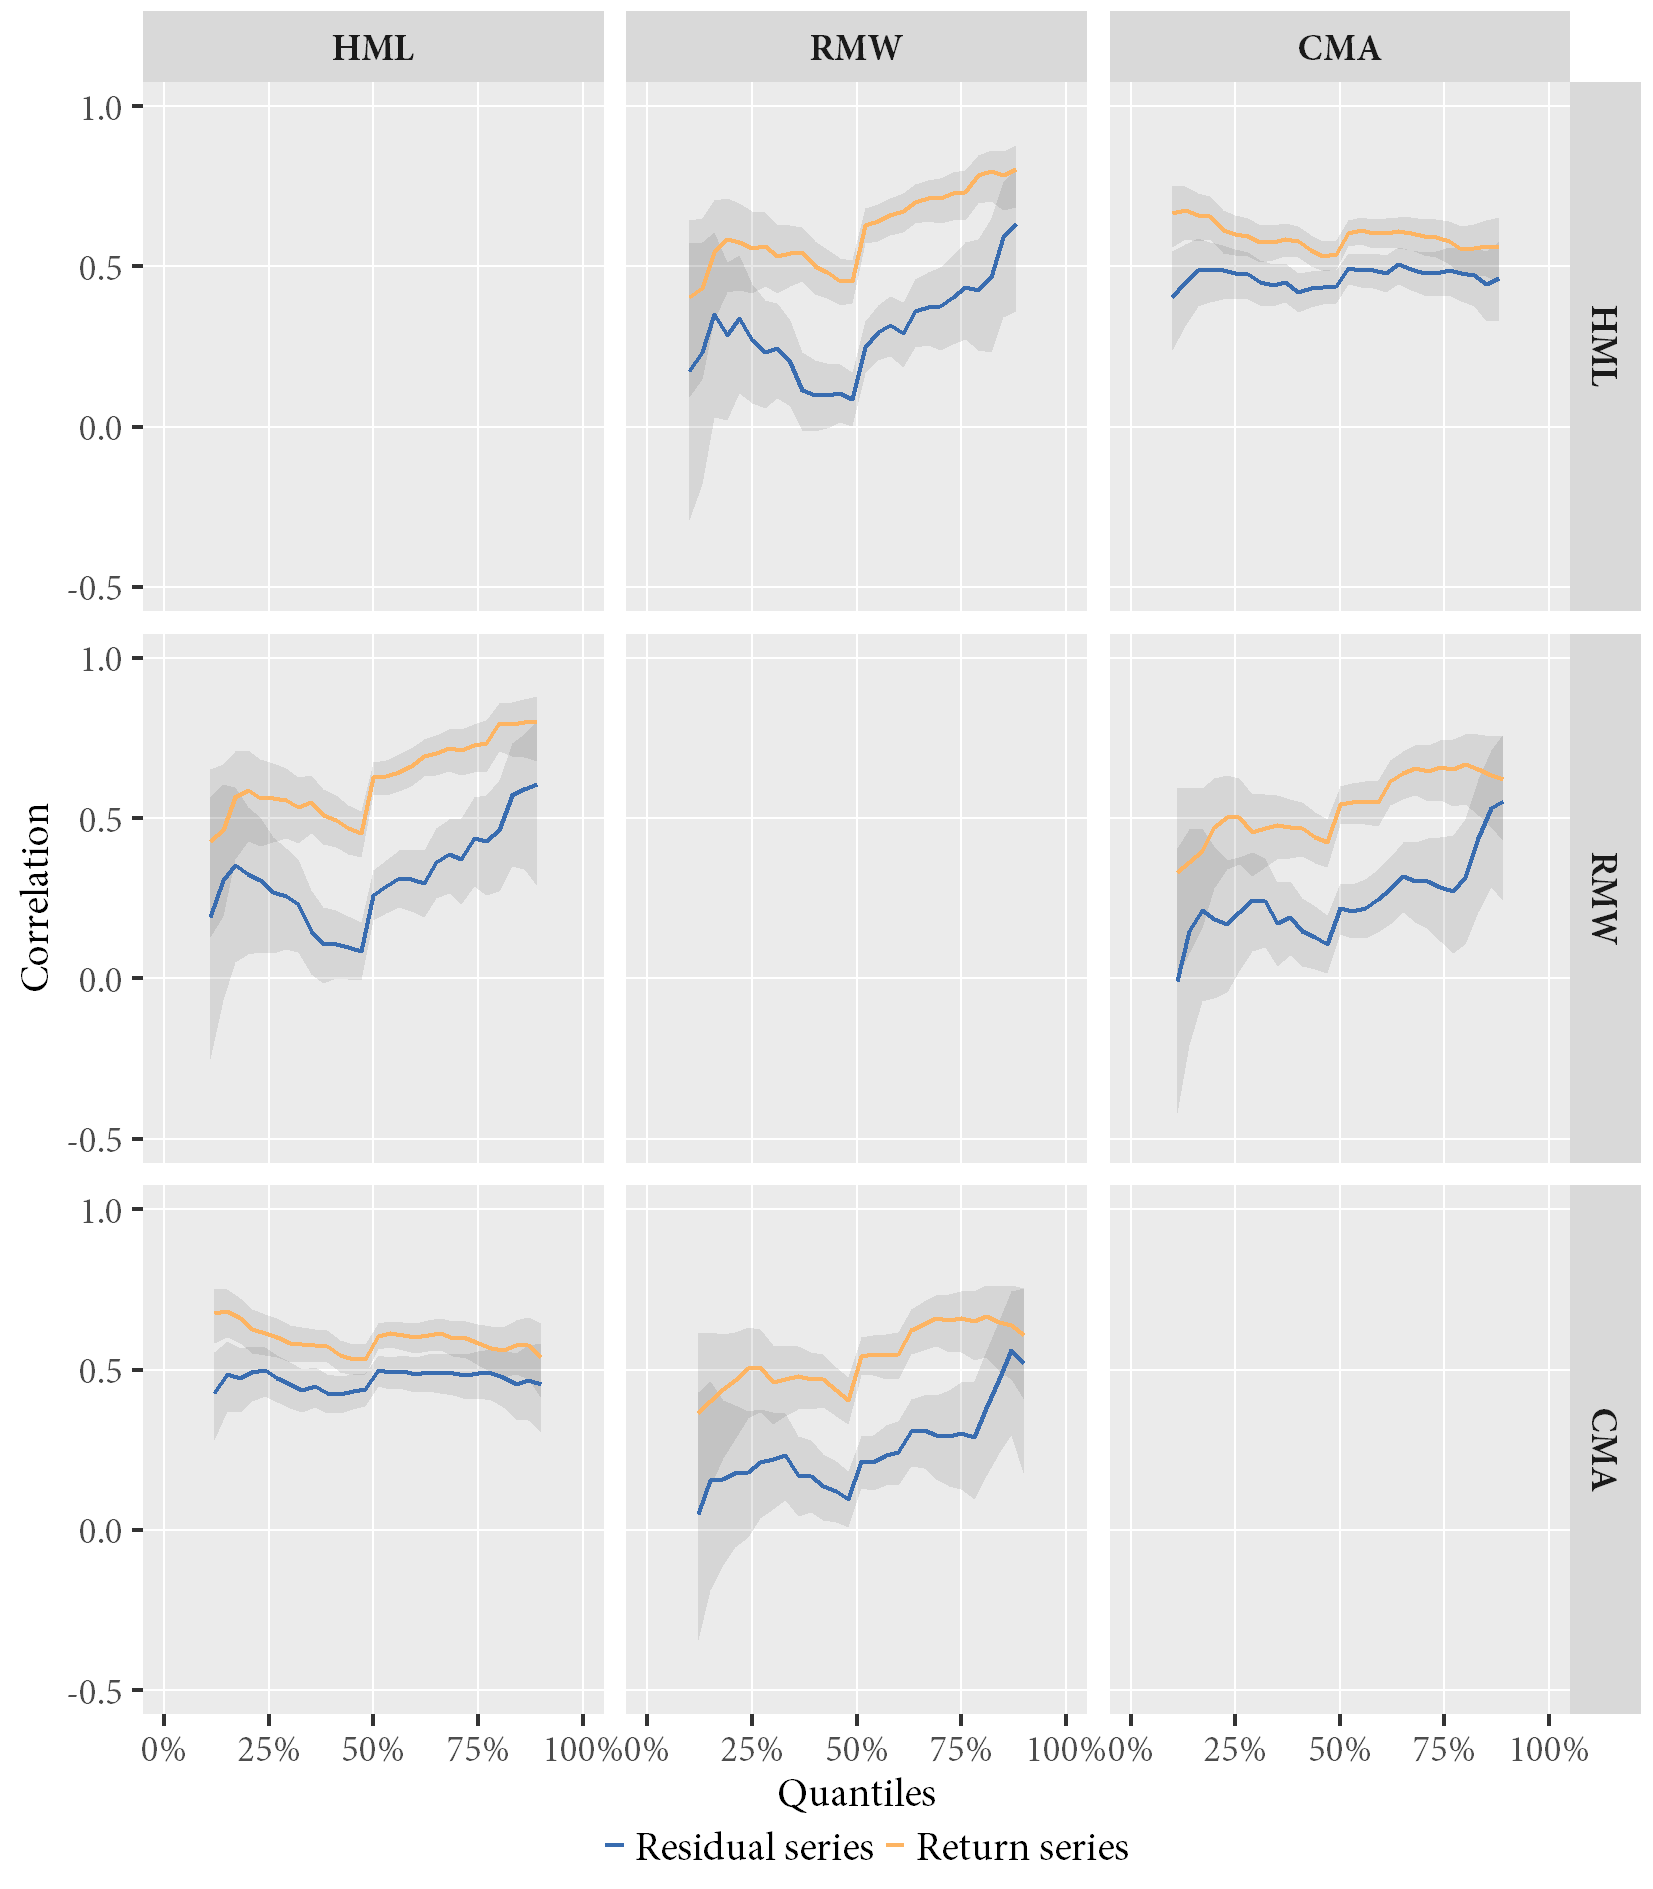
\includegraphics[scale=1]{graphics/threshold_Value.png}  
  % \bottomrule
  \vspace{3mm}
  \footnotesize
  We report threshold correlations of factor strategy pairs. Return series are weekly log returns and residual series are weekly standardized residuals from an ARMA-GJR-GARCH process. Value factors in columns and rows. All data 1963-07-05 - 2016-07-01. Correlations from 10-90\% reported, due to limited data availablility in the tails. Threshold correlations are calculated as: $Corr(r_i, r_j \,|\, r_i < F_i^{-1}(p), r_j < F_j^{-1}(p)) \text{ for } p < 0.5$ and $Corr(r_i, r_j \,|\, r_i \geq F_i^{-1}(p), r_j \geq F_j^{-1}(p)) \text{ for } p \geq 0.5$
  \end{minipage}
\end{figure}

\begin{itemize}
  \item There is a marked difference between the threshold correlations before and after applying a GARCH filter. We conclude that a large part of what intially seems as multivariate asymmetry is in fact due to simultaneous ARMA-GARCH effects on the marginal level (see~\autoref{diag:thresholdnonvalue})
  \item Still, there is a lot of tail dependence and asymmetry left. A Gaussian model with linear correlations approaches zero correlation when the quantile goes to zero and one respectively. Particularly between value factors (see~\autoref{diag:thresholdvalue}), there is both marked asymmetry and tail dependency in the residual series.
  \item Considering~\autoref{diag:thresholdnonvalue}, the correlation between Market and HML is increasing in the lower quantiles -- opposite what you want. This could be indicative that HML offers poor protection in bad times, the increased recession risk being part of the traditional explanation behind the value premium.
\end{itemize}
\subsection{Copula results}
% TABLES NEED TO BE MODIFIED IN THE FOLLOWING WAYS
% 1) Change {tabular} to {tabularx}{\textwidth} and make leftmost column an X column
%     and change top and bottom \hline to \toprule \bottomrule
%
% paste the following at start but before & \multicolumn
%
% \begin{tabularx}{\textwidth}{@{\extracolsep{5pt}} X D{.}{.}{-3} D{.}{.}{-3} D{.}{.}{-3} } 
% \\[-1.8ex] \midrule
% \\[-1.8ex] 
%
% paste the following at end after R2 row but before Note row
% \bottomrule \\[-1.8ex] 
%
% 2) Change the variable names to greeks
% 3) Change specification names if needed
% 4) Change R2 to LLH and add similar lines for Ljung-Box and ARCH-LM
% 5) Add label and caption
% 6) Paste this to get table heading description
% 7) Copy table heading tabularx footnote size text
%
% \begin{tabularx}{\textwidth}{X}
% \\[-1.8ex]\toprule
%\\[-1.8ex] 
% text goes here
% \end{tabularx}
%
% 6) Copy the whole table, only change caption, label, factor/spec labels and (1)-(3) to (4)-(6)
% Table created by stargazer v.5.2 by Marek Hlavac, Harvard University. E-mail: hlavac at fas.harvard.edu
% Date and time: ons, okt 12, 2016 - 12:37:02
% Requires LaTeX packages: dcolumn 
\begin{table}[!htbp] \centering 
  \caption{Copula results: Constant specifications} 
  \label{tab:copula1} 
\begin{tabularx}{\textwidth}{X}
  \\[-1.8ex]\toprule
  \\[-1.8ex] 
  \footnotesize Parameter estimates from constant copula models based on uniform residuals from ARMA-GJR-GARCH models. Stationary bootstrap standard errors in parentheses, following \textcite{PolitisRomano1994}. Copula parameters: $\nu$ is the degree of freedom, $\gamma$ is the vector of skewness parameters, $\alpha, \beta$ are the shock loading and autoregressive loading of the \textit{c}DCC process. All data 1963-07-05 - 2016-07-01. 
\end{tabularx}
\begin{tabularx}{\textwidth}{@{\extracolsep{5pt}} X D{.}{.}{-3} D{.}{.}{-3} D{.}{.}{-3} } 
  \\[-1.8ex]\midrule
  \\[-1.8ex] 
   & \multicolumn{3}{c}{Constant copula models} \\ 
  \cline{2-4} 
  \\[-1.8ex] & \multicolumn{1}{c}{(1)} & \multicolumn{1}{c}{(2)} & \multicolumn{1}{c}{(3)}\\ 
  \\[-1.8ex] & \multicolumn{1}{c}{Gaussian} & \multicolumn{1}{c}{Student-\textit{t}} & \multicolumn{1}{c}{Skewed Student-\textit{t}}\\ 
  \hline \\[-1.8ex] 
 $\nu$ &  & 6.656 & 6.707 \\ 
  &  & () & () \\ 
  & & & \\ 
 $\gamma_{Mkt.RF}$ &  &  & -0.034 \\ 
  &  &  & () \\ 
  & & & \\ 
 $\gamma_{HML}$ &  &  & 0.103 \\ 
  &  &  & () \\ 
  & & & \\ 
 $\gamma_{SMB}$ &  &  & -0.102 \\ 
  &  &  & () \\ 
  & & & \\ 
 $\gamma_{Mom}$ &  &  & -0.183 \\ 
  &  &  & () \\ 
  & & & \\ 
 $\gamma_{RMW}$ &  &  & 0.019 \\ 
  &  &  & () \\ 
  & & & \\ 
 $\gamma_{CMA}$ &  &  & 0.086 \\ 
  &  &  & () \\ 
  & & & \\ 
 $\alpha$ & 0 & 0 & 0 \\ 
  &  &  &  \\ 
  & & & \\ 
 $\beta$ & 0 & 0 & 0 \\ 
  &  &  &  \\ 
  & & & \\ 
\hline \\[-1.8ex] 
Observations & \multicolumn{1}{c}{2,766} & \multicolumn{1}{c}{2,766} & \multicolumn{1}{c}{2,766} \\ 
LLH & \multicolumn{1}{c}{1,170} & \multicolumn{1}{c}{1,550} & \multicolumn{1}{c}{1,564} \\ 
No. parameters & \multicolumn{1}{c}{15} & \multicolumn{1}{c}{16} & \multicolumn{1}{c}{22} \\ 
BIC & \multicolumn{1}{c}{-2,222} & \multicolumn{1}{c}{-2,972} & \multicolumn{1}{c}{-2,954} \\ 
Correlation $(Q)$ persistence $(\alpha+\beta)$ & \multicolumn{1}{c}{0} & \multicolumn{1}{c}{0} & \multicolumn{1}{c}{0} \\ 
\bottomrule \\[-1.8ex] 
\textit{Note:}  & \multicolumn{3}{c}{$^{*}$p$<$0.1; $^{**}$p$<$0.05; $^{***}$p$<$0.01} \\ 
\end{tabularx} 
\end{table} 
% Table created by stargazer v.5.2 by Marek Hlavac, Harvard University. E-mail: hlavac at fas.harvard.edu
% Date and time: ons, okt 12, 2016 - 12:37:02
% Requires LaTeX packages: dcolumn 
\begin{table}[!htbp] \centering 
  \caption{Copula results: \textit{c}DCC specifications} 
  \label{tab:copula2} 
\begin{tabularx}{\textwidth}{X}
\\[-1.8ex]\toprule
\\[-1.8ex] 
\footnotesize Parameter estimates from dynamic copula models based on uniform residuals from ARMA-GJR-GARCH models. Stationary bootstrap standard errors in parentheses, following \textcite{PolitisRomano1994}. Copula parameters: $\nu$ is the degree of freedom, $\gamma$ is the vector of skewness parameters, $\alpha, \beta$ are the shock loading and autoregressive loading of the \textit{c}DCC process. All data 1963-07-05 - 2016-07-01. 
\end{tabularx}
\begin{tabularx}{\textwidth}{@{\extracolsep{5pt}} X D{.}{.}{-3} D{.}{.}{-3} D{.}{.}{-3} } 
\\[-1.8ex]\midrule
\\[-1.8ex] 
 & \multicolumn{3}{c}{Dynamic copula models} \\ 
\cline{2-4} 
\\[-1.8ex] & \multicolumn{1}{c}{(4)} & \multicolumn{1}{c}{(5)} & \multicolumn{1}{c}{(6)}\\ 
\\[-1.8ex] & \multicolumn{1}{c}{Gaussian} & \multicolumn{1}{c}{Student-\textit{t}} & \multicolumn{1}{c}{Skewed Student-\textit{t}}\\ 
\hline \\[-1.8ex] 
 $\nu$ &  & 11.831 & 11.803^{***} \\ 
  &  & () & (1.064) \\ 
  & & & \\ 
 $\gamma_{Mkt.RF}$ &  &  & -0.055 \\ 
  &  &  & (0.054) \\ 
  & & & \\ 
 $\gamma_{HML}$ &  &  & 0.071 \\ 
  &  &  & (0.058) \\ 
  & & & \\ 
 $\gamma_{SMB}$ &  &  & -0.170^{**} \\ 
  &  &  & (0.077) \\ 
  & & & \\ 
 $\gamma_{Mom}$ &  &  & -0.125^{*} \\ 
  &  &  & (0.073) \\ 
  & & & \\ 
 $\gamma_{RMW}$ &  &  & 0.095 \\ 
  &  &  & (0.061) \\ 
  & & & \\ 
 $\gamma_{CMA}$ &  &  & 0.022 \\ 
  &  &  & (0.063) \\ 
  & & & \\ 
 $\alpha$ & 0.066 & 0.068 & 0.068^{***} \\ 
  & () & () & (0.007) \\ 
  & & & \\ 
 $\beta$ & 0.915 & 0.913 & 0.913^{***} \\ 
  & () & () & (0.011) \\ 
  & & & \\ 
\hline \\[-1.8ex] 
Observations & \multicolumn{1}{c}{2,766} & \multicolumn{1}{c}{2,766} & \multicolumn{1}{c}{2,766} \\ 
LLH & \multicolumn{1}{c}{2,791} & \multicolumn{1}{c}{2,975} & \multicolumn{1}{c}{2,984} \\ 
No. parameters & \multicolumn{1}{c}{17} & \multicolumn{1}{c}{18} & \multicolumn{1}{c}{24} \\ 
BIC & \multicolumn{1}{c}{-5,448} & \multicolumn{1}{c}{-5,807} & \multicolumn{1}{c}{-5,778} \\ 
Correlation $(Q)$ persistence $(\alpha+\beta)$ & \multicolumn{1}{c}{0.980} & \multicolumn{1}{c}{0.981} & \multicolumn{1}{c}{0.981} \\ 
\bottomrule \\[-1.8ex] 
\textit{Note:}  & \multicolumn{3}{c}{$^{*}$p$<$0.1; $^{**}$p$<$0.05; $^{***}$p$<$0.01} \\ 
\end{tabularx} 
\end{table} 

\begin{figure}[H]
  \caption{Constant Copula Threshold Correlations - Value factors vs. non-value factors}
  \label{diag:thresholdnonvalue_copula}
  % \toprule
  \centering
  \begin{minipage}{\textwidth}
  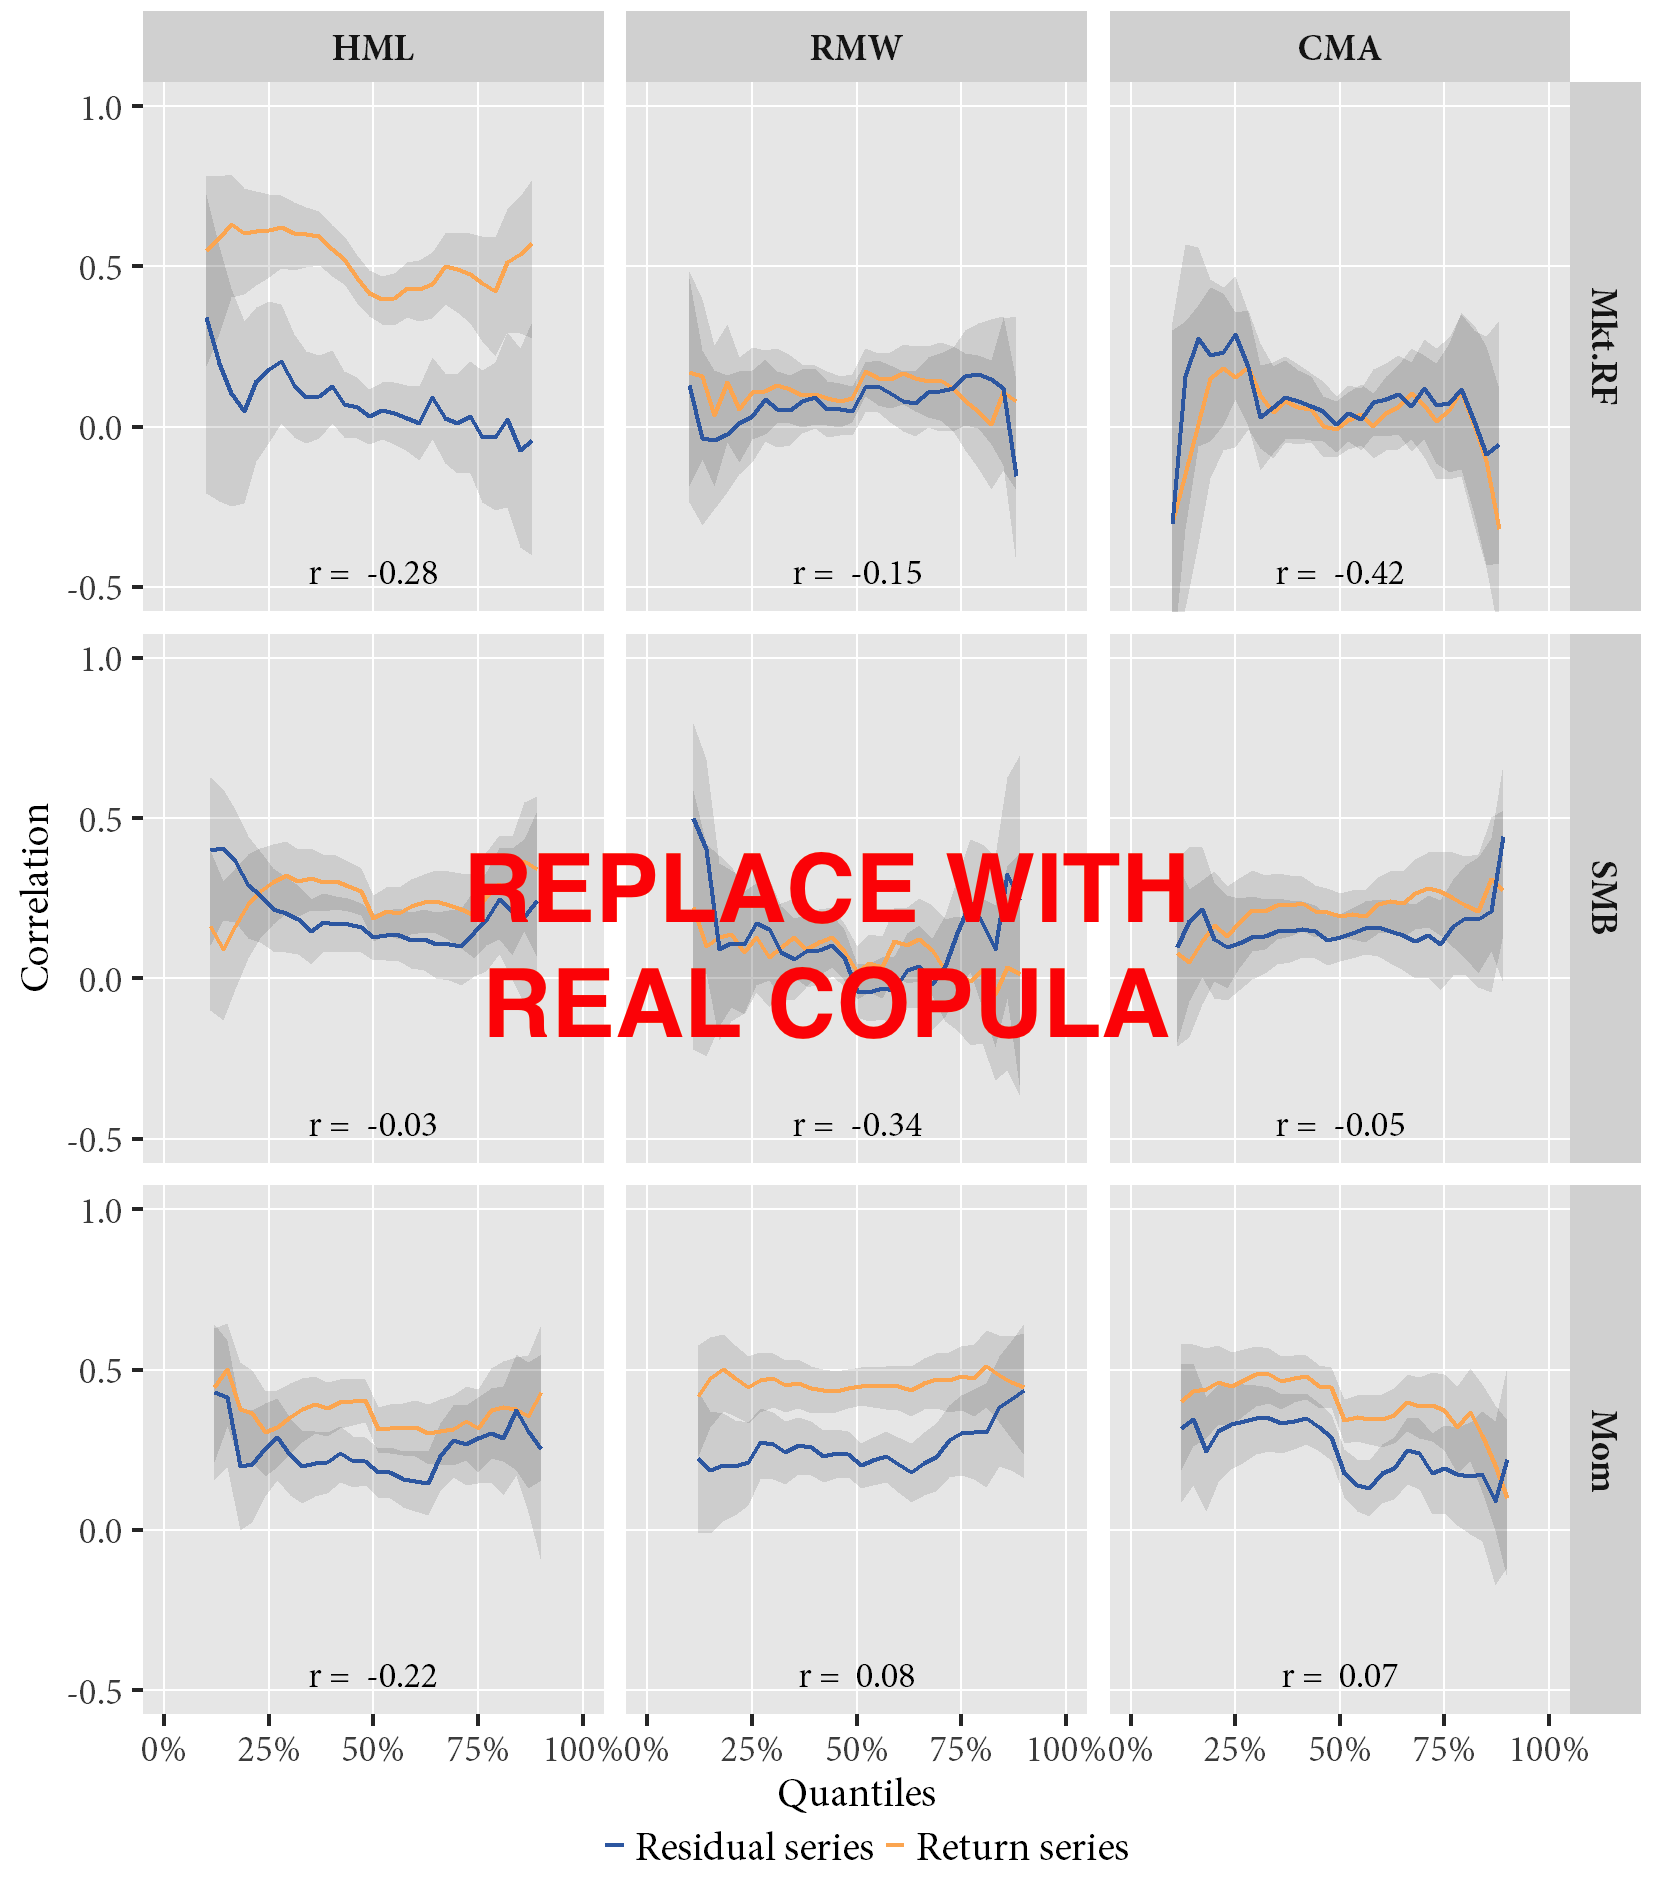
\includegraphics[scale=1]{graphics/threshold_Nonvalue_copula.png}  
  % \bottomrule
  \vspace{3mm}
  \footnotesize
  We report threshold correlations on standardized residuals, empirical filtered from GARCH and simulated from constant copula models. Value factors in columns and non-value factors in rows. All data 1963-07-05 - 2016-07-01. Correlations from 10-90\% reported, due to limited data availablility in the tails. Threshold correlations are calculated as: $Corr(r_i, r_j \,|\, r_i < F_i^{-1}(p), r_j < F_j^{-1}(p)) \text{ for } p < 0.5$ and $Corr(r_i, r_j \,|\, r_i \geq F_i^{-1}(p), r_j \geq F_j^{-1}(p)) \text{ for } p \geq 0.5$ 
  \end{minipage}
\end{figure}
\begin{figure}[H]
  \caption{Constant Copula Threshold Correlations - Value factors vs. themselves}
  \label{diag:thresholdvalue_copula}
  % \toprule
  \centering
  \begin{minipage}{\textwidth}
  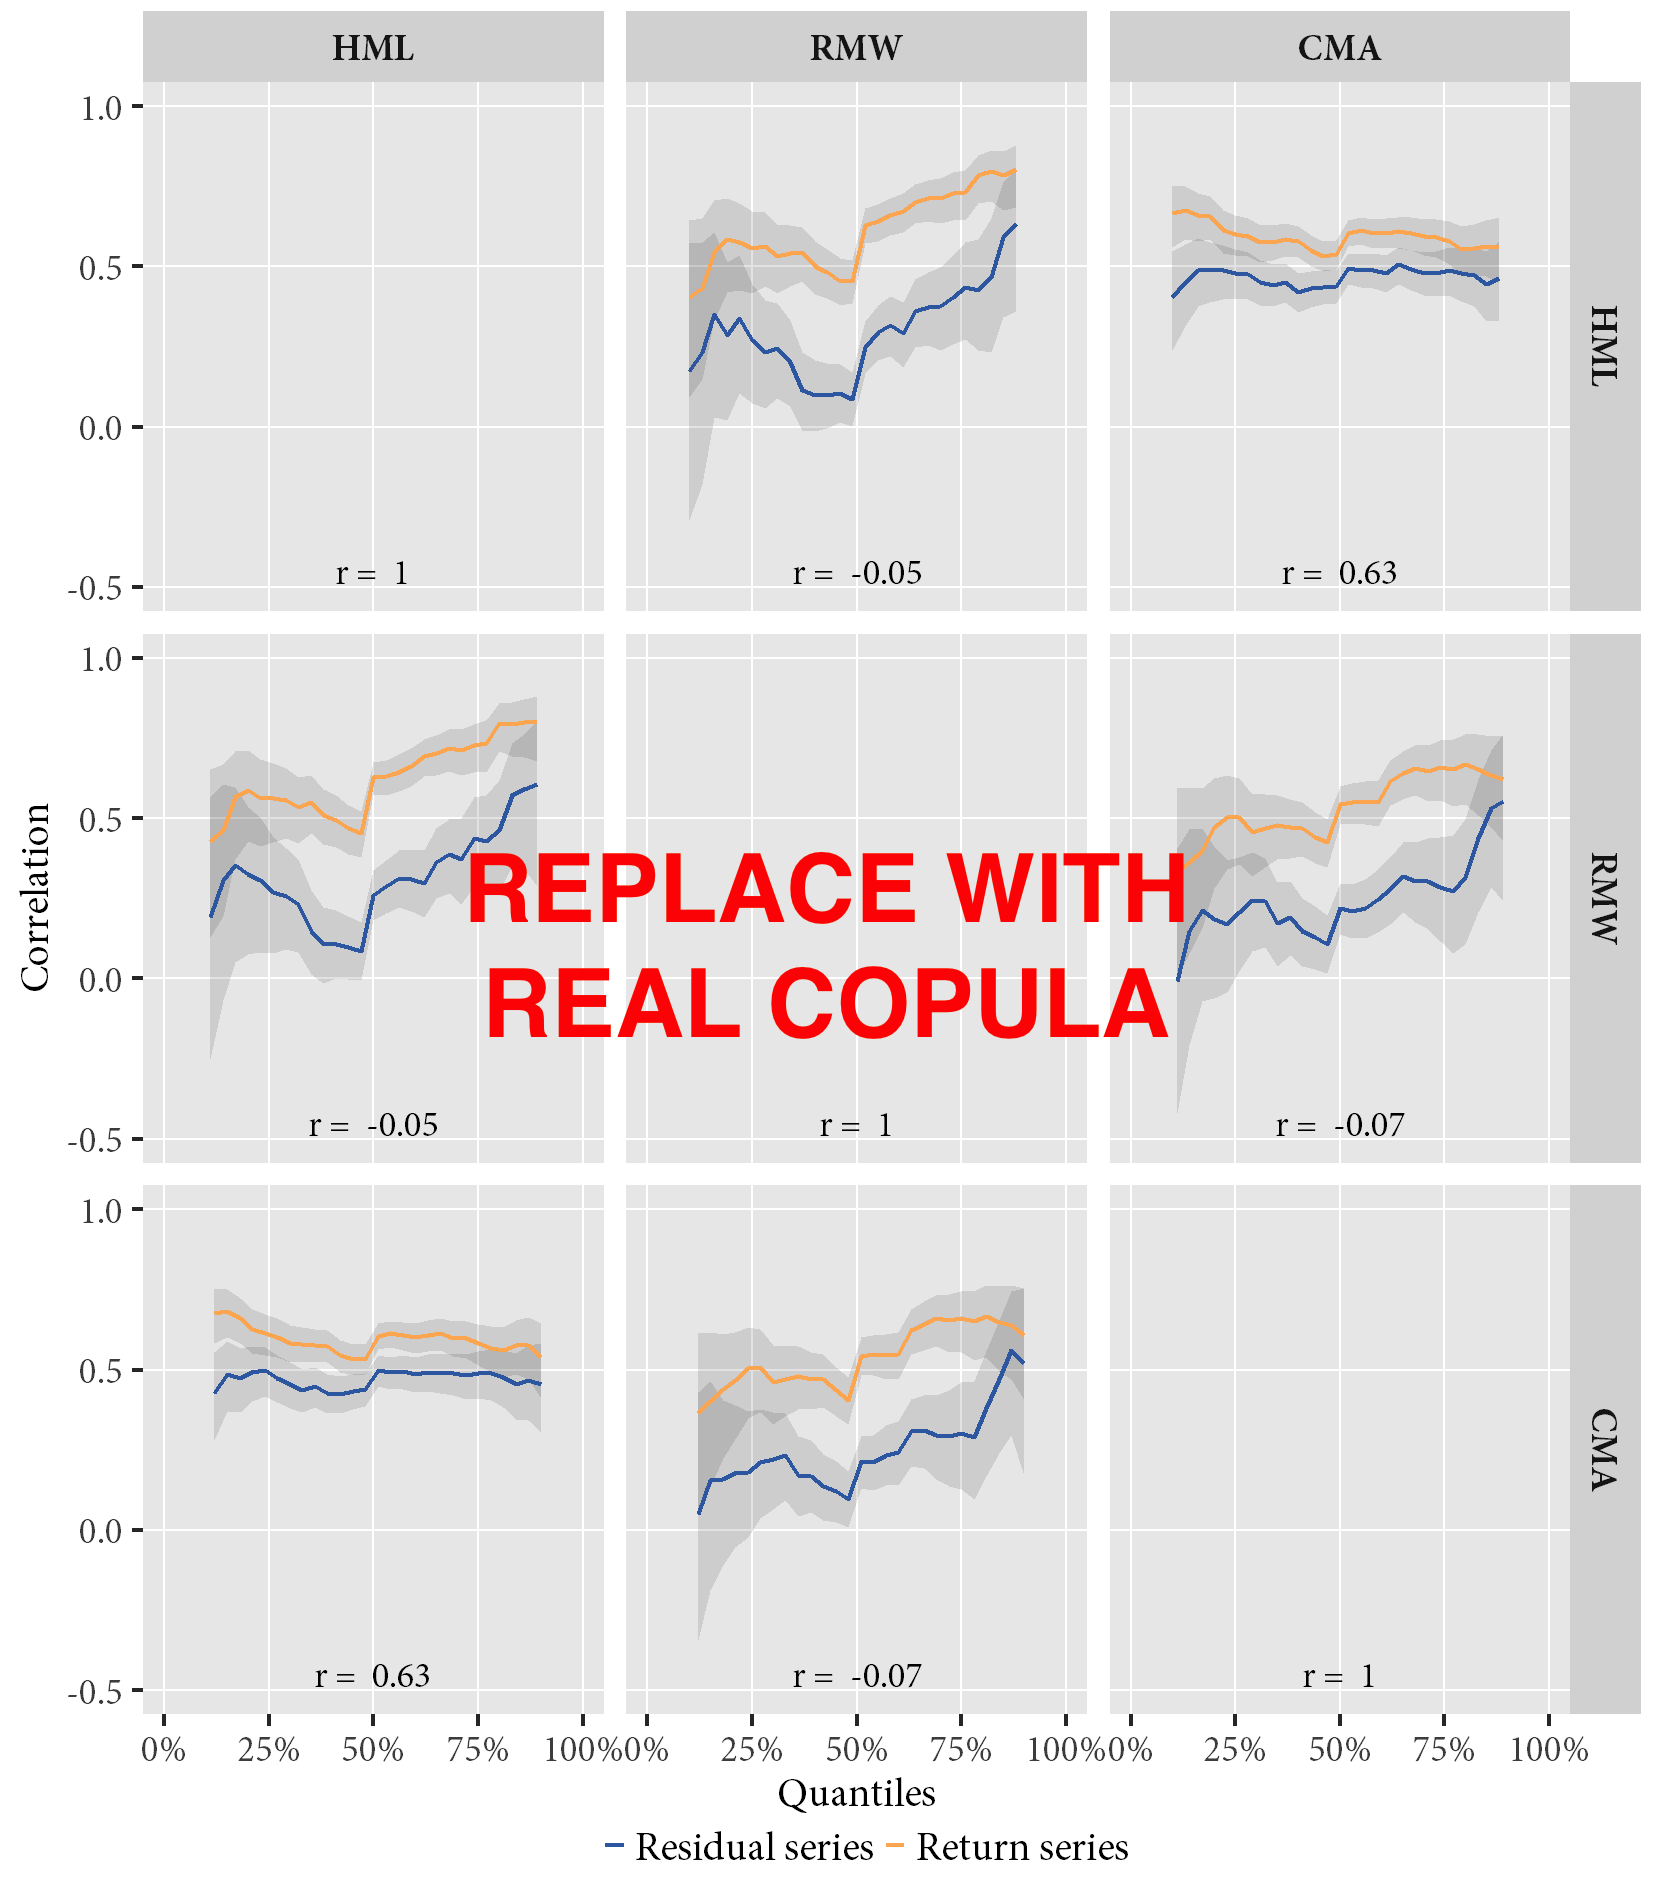
\includegraphics[scale=1]{graphics/threshold_Value_copula.png}  
  % \bottomrule
  \vspace{3mm}
  \footnotesize
  We report threshold correlations on standardized residuals, empirical filtered from GARCH and simulated from constant copula models. Value factors against each other. All data 1963-07-05 - 2016-07-01. Correlations from 10-90\% reported, due to limited data availablility in the tails. Threshold correlations are calculated as: $Corr(r_i, r_j \,|\, r_i < F_i^{-1}(p), r_j < F_j^{-1}(p)) \text{ for } p < 0.5$ and $Corr(r_i, r_j \,|\, r_i \geq F_i^{-1}(p), r_j \geq F_j^{-1}(p)) \text{ for } p \geq 0.5$ 
  \end{minipage}
\end{figure}

\begin{itemize}
  \item Looking at threshold correlations of the constant copula models (see~\autoref{diag:thresholdnonvalue_copula} and \autoref{diag:thresholdvalue_copula}), we see that the asymmetric copula can approach to capture some of the important asymmetric patterns. The Gaussian copula's threshold correlations fail to do so.
  \item Log-likelihood is strongly improved by estimating a dynamic copula -- dependency appears to vary over time (see~\autoref{diag:rolling_copula}). 
  \item Asymmetry parameters are not very significant (note: we need to bootstrap more values to get proper standard errors). The improvement in log-likelihood from symmetric to skewd Student's t is not very large. A lot of asymmetry is apparently taken care of at the marginal level; importance of asymmetric tail dependency diminished. BIC statistic also prefers symmetric Student's t -- asymmetric introduces 6 additional parameters.
  \item Sum of $\alpha$ and $\beta$ is high so that correlation does not return quickly to ``average'' level -- near unit root.
\end{itemize}

\begin{figure}[H]
  \caption{Copula Correlations - Value factors vs. all factors}
  \label{diag:rolling_copula}
  % \toprule
  \centering
  \begin{minipage}{\textwidth}
  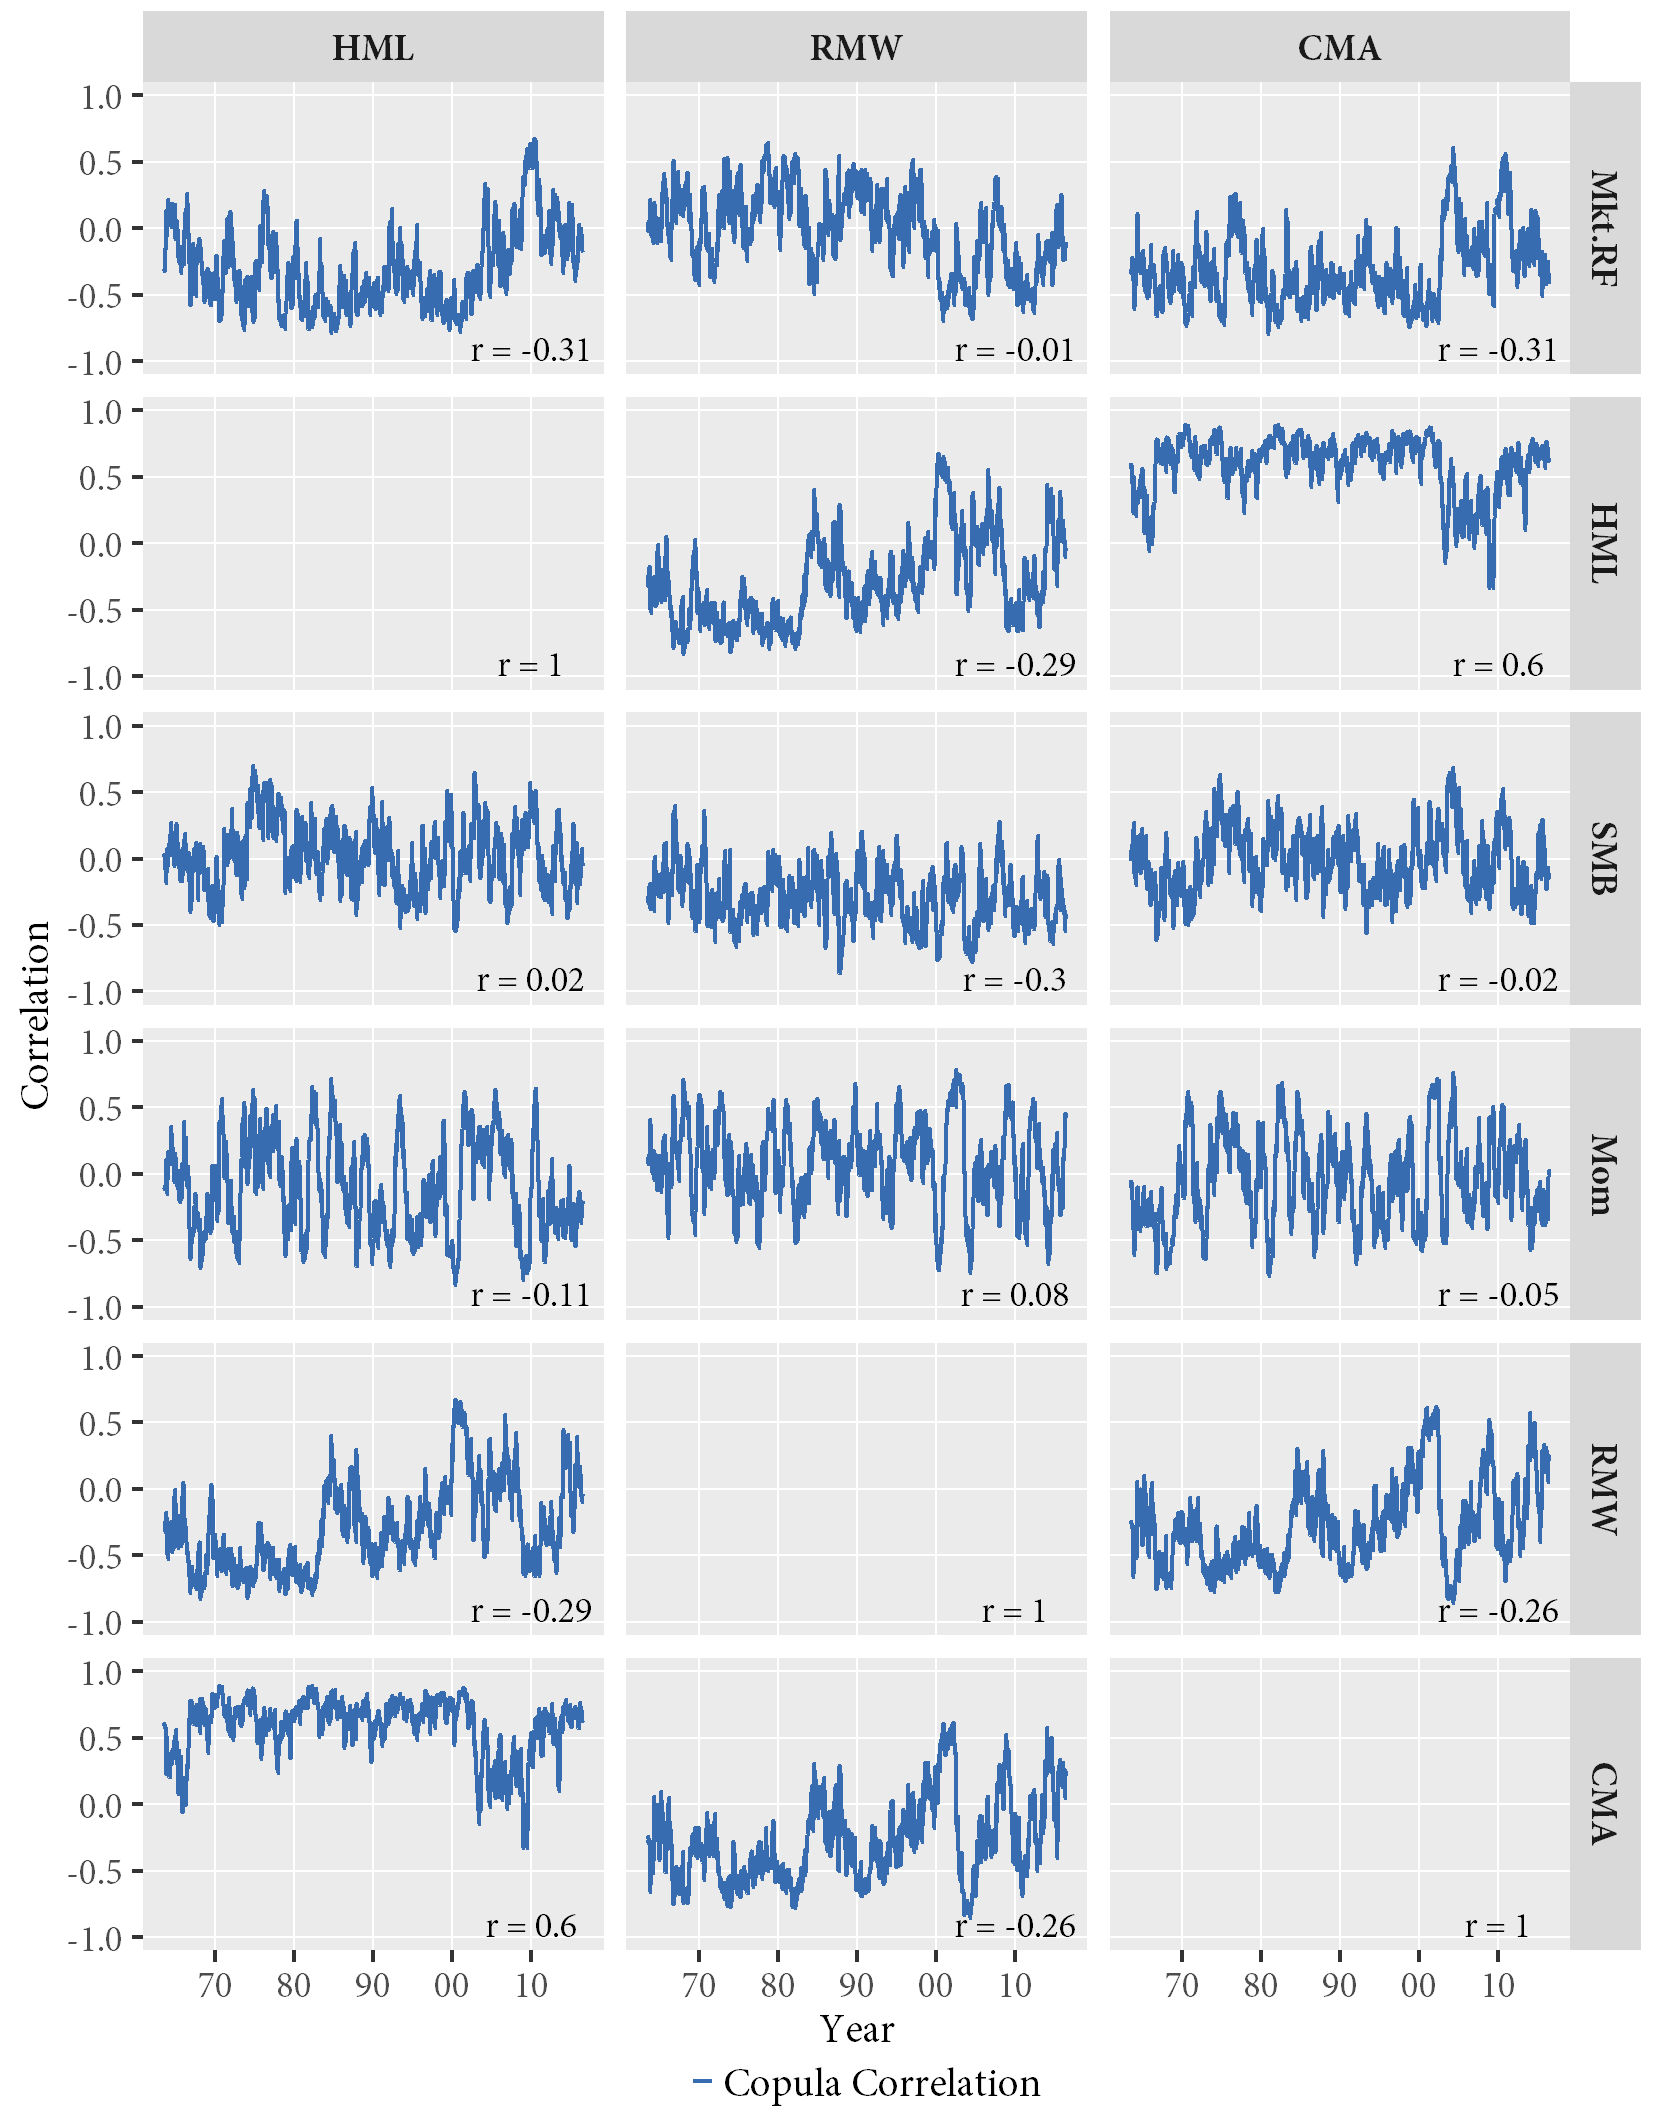
\includegraphics[scale=1]{graphics/rolling_copula_ghskt.png}  
  % \bottomrule
  \vspace{3mm}
  \footnotesize
  We report the conditional correlation matrix from the dynamic skewed Student's copula estimated on the full dataset. The standard correlation coefficient refers to correlation of the time-invariant component ($S$). All data 1963-07-05 - 2016-07-01.
  \end{minipage}
\end{figure}

\subsection{Conditional diversification benefit}
\begin{figure}[H]
  \caption{Conditional diversification benefit of different strategies}
  \label{diag:cdb1}
  % \toprule
  \centering
  \begin{minipage}{\textwidth}
  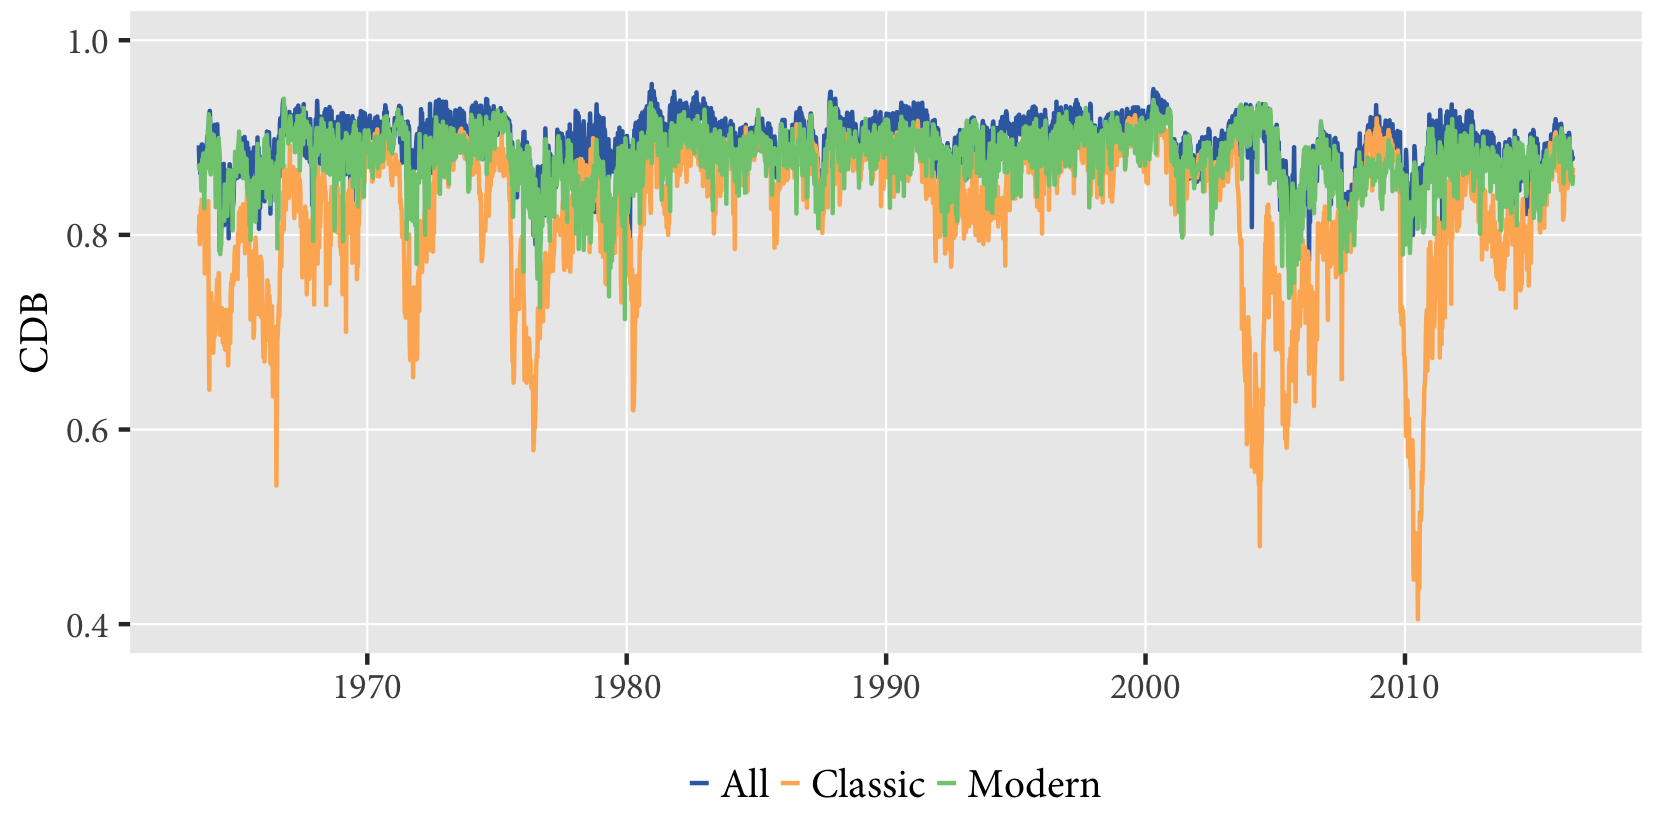
\includegraphics[width=\textwidth]{graphics/cdb--modern-classic.png}  
  % \bottomrule
  \vspace{3mm}
  \footnotesize
  We report conditional diversification benefit of three asset universes: All (including $Mkt.RF$, $HML$, $SMB$, $Mom$, $RMW$, $CMA$), Classic (All excluding $RMW$, $CMA$), and Modern (All excluding $HML$). A value closer to one indicates greater diversification benefit and a value of zero indicates no diversification benefit. All data 1963-07-05 - 2016-07-01, using simulations from the copula model.
  \end{minipage}
\end{figure}

\begin{figure}[H]
  \caption{CDB with RMW combined with HML or CMA}
  \label{diag:cdb--rmw_cma-rmw_hml}
  % \toprule
  \centering
  \begin{minipage}{\textwidth}
  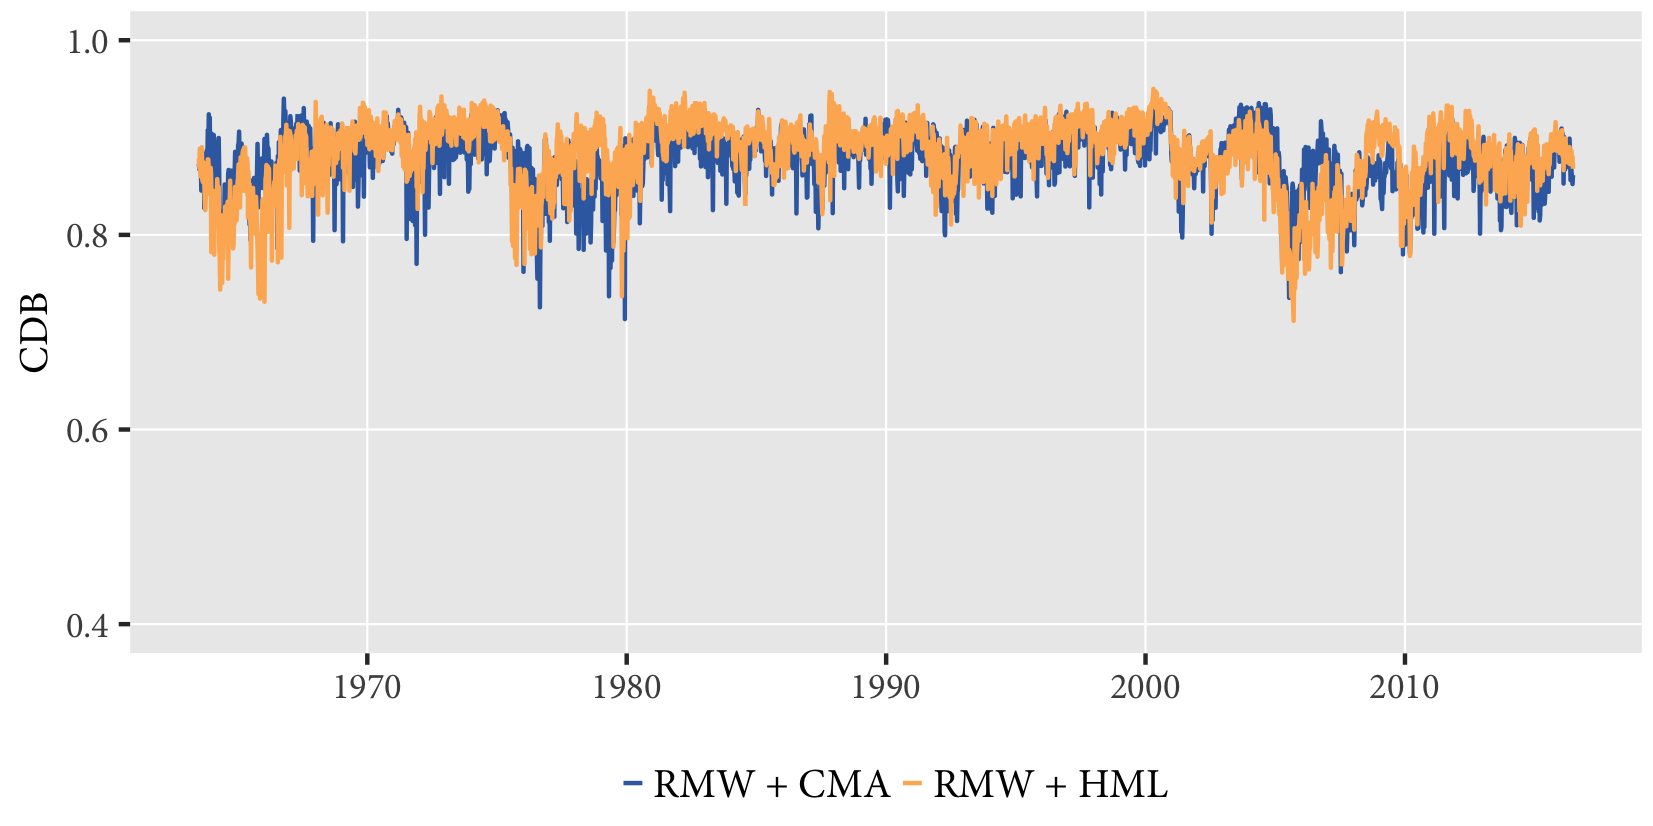
\includegraphics[width=\textwidth]{graphics/cdb--rmw_cma-rmw_hml.png}  
  % \bottomrule
  \vspace{3mm}
  \footnotesize
  We report CDB from portfolios built using non-value factors (Market, SMB and Momentum) and a combination of RMW and CMA or RMW and HML. A value closer to one indicates greater diversification benefit and a value of zero indicates no diversification benefit. All data 1963-07-05 - 2016-07-01, using simulations from the copula model.
  \end{minipage}
\end{figure}

\begin{figure}[H]
  \caption{CDB with one value factor at a time (RMW, CMA, HML)}
  \label{diag:cdb--rmw-cma-hml}
  % \toprule
  \centering
  \begin{minipage}{\textwidth}
  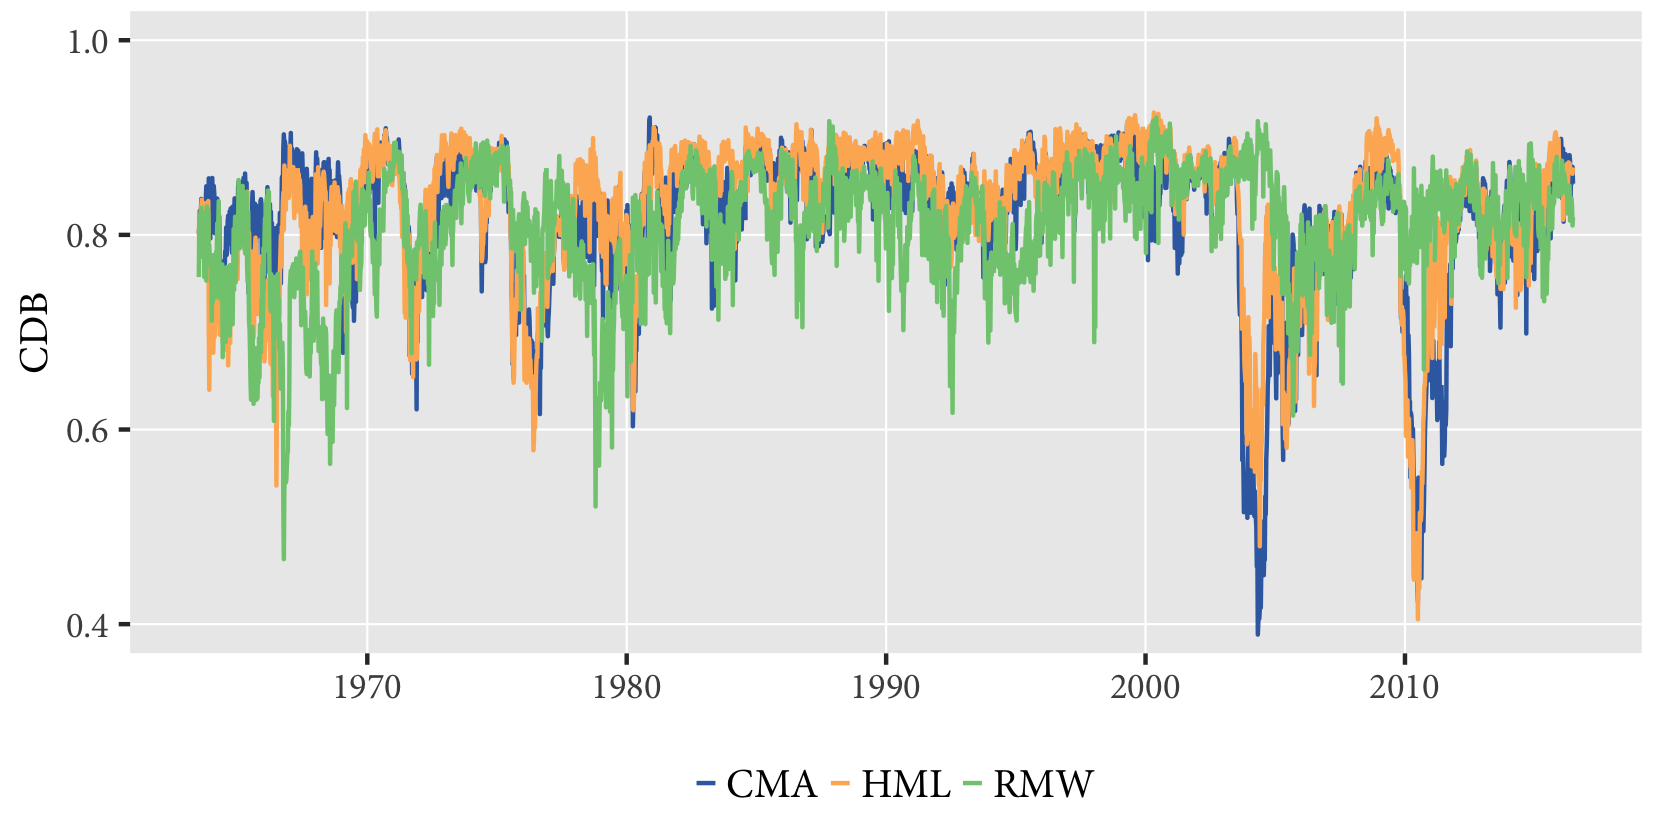
\includegraphics[width=\textwidth]{graphics/cdb--rmw-cma-hml.png}
  % \bottomrule
  \vspace{3mm}
  \footnotesize
  We report CDB from portfolios built using non-value factors (Market, SMB and Momentum) and one value factor (CMA, RMW or HML). A value closer to one indicates greater diversification benefit and a value of zero indicates no diversification benefit. All data 1963-07-05 - 2016-07-01, using simulations from the copula model.
  \end{minipage}
\end{figure}

\begin{itemize}
  \item Looking at~\autoref{diag:cdb1}, if we take a portfolio consisting of ``modern'' value as our benchline, there appears to be little improvement in conditional diversification benefit by adding HML (``all''). On the contrary, in a portfolio not including RMW or CMA (``classic''), the optimal level of diversification benefit is often considerably lower than the modern or full portfolio. That modern value outperforms classic is perhaps not surprising (you have one additional asset to diversify into), however.
  \item There are some notable failures of classic value by looking at~\autoref{diag:cdb1}, for crisis years 1973--1976, 1999--2001 and 2008--2010. It appears that not holding RMW or CMA can be especially problematic in such times.
  \item Given the high correlation between HML and CMA, it's relevant to consider portfolios combining RMW with HML or CMA, see~\autoref{diag:cdb--rmw_cma-rmw_hml}. Based on this image, it's not obvious that HML is redundant. On average, CDB of RMW+HML is 0.05 higher than HML+CMA.
  \item \autoref{diag:cdb--rmw-cma-hml} shows portfolios using just one value factor. Based on this image, it appears that RMW is not the great diversifer on its own -- it needs HML or CMA to be effective (with HML, from the previous picture, outperforming).
\end{itemize}
